% !TeX root = ../main.tex
% !TeX spelling = en_GB
% !TeX program = pdflatex

\chapter{Discussion}
\label{chap:discussion}



\section{Starting Studies}



\subsection{Infrared and Visible Light}

The amound of absorbed light in a small water droplet is close to negligible compared to the scattered light. In a large ensemble of droplets, such as a cloud, the total absorption will still be significant, especially for wavelengths in the near and far infrared. Since it was possile, we made a quick comparison of illumination using blue light (ca 450nm) and near infrared (ca 850nm). The blue light gave the sharpest image, probably due to the sensor's slightly higher sensitivity for blue light. But also possibly due to the higher theoretical resolving power as described by Rayleigh's criterion. See Paper I.

\subsection{Laser Light}

Lasers are used in most optical instruments for droplet measurement and for many good reasons. Prices for high power semiconductor lasers have also become very attractive. The coherency gives the possibility of using holographic reconstruction of diffraction patterns to achieve a larger measuring range than what is possible in conventional imaging. Sizing of particles may still be tricky, and especially more calculation intensive. For conventional imaging of small particles the coherence mainly causes problems as the diffraction patterns will be strong and visible. Although it is possbile to make the laser incoherent e.g. by using diffusers or optical fibres it is still another circumstance that makes the complete system slightly more complex.

\subsection{Image Noise and SNR}

The design using a weakly collimated LED that illuminates an area slightly larger than the field of view makes the system quite insensitive to misalignment of the camera and the light source. Temporal or permanent changes in light intensity caused by a minor misalignment can be automatically compensated for by continuous measurement of the total exposure level. If the level of exposure is increasing or decreasing, the length of the light pulse is changed correspondingly. The light intensity can also be affected by dirt on the front glass of the housings. 

Spatial dissimilarities in the light intensity that are not caused by noise we can compensate for by calculating the local average intensity of the background around each measured droplet. The size of a droplet is then based on the intensity dip caused by the shadow compared with its local background.

\subsection{Image Pre-processing}

To increase the number of processed images a pre-process is done using a variable threshold as described in section \ref{imgsegment}. The processing speed could be increased even more limiting the edge detection algorithm to the region or regions around the discovered differences.

\subsection{Light Sensitivity Measurement}

This measurement was done to get an idea about the theoretical minimum amount of energy required for each image. In practice, the light from the collimated LED used will be spread so that only a small part of the total emitted energy actually reaches the sensor. The area in view is about 8 times smaller than the illuminated area of the collimated LED, which was measured to about 8x8 mm. Also a lot of the light energy will be absorbed in the telecentric lens.

\subsection{Speed of Light Flash}

the illuminative power need to be enough to get a good exposure at a high wind speeds.
The LED used was fully functional after four months of continous measurements using 12 times higher current than specified. Using even higher current 

\section{Aerodynamics}

Many existing instruments suffer from errors caused by the instrument itself during sampling, e.g. when droplets get stuck on the inlet or shatters into smaller droplets. The DII is not as small and aerodynamically shaped as the \gls{cdp}, therefore a difference between the instruments would be expected depending on the air speed. However, a comparison between the measured values of LWC showed no connection between the wind speed and the difference in the measured LWC. The wind speed during the comparison was only 1-4 $\mathrm{m \cdot s^{-1}}$ which probably explain why the less aerodynamic shape of the DII compared with the \gls{cdp} has no noticeable effect. This could change dramatically when measuring at higher wind speeds.

\section{Difficulties with Polymer Microspheres}

To verifiy the sizing algorithm, a measurement using polymer microspheres of four known calibrated size distributions was done. To simulate real conditions as much as possible the microspheres were applied using the same dispenser used for the calibration of the \gls{cdp}. The smallest microspheres had a tendency of clogging leading sometimes to a measurement of a clog as a single particle. Therefore all images were visually checked for false measurements. The outliers caused by false measurements were removed.

\subsection{Clogging}

Small microspheres are forming larger clogs that are measured as single microspheres. The reason may be static electricity or humidity. As can be seen in the five micrometer measurement, the result of some clogs becomes outliers in the expected distribution. This needs to be considered when solid microspheres are used as reference objects. Colliding liquid water droplets would of course coalesce into larger droplets, thereby changing the diameter.

The equipment and the dispenser was thoroughly cleaned using compressed air between each measurement. Still there may be microspheres or other contamination left, changing the distribution slightly.

Measured mean and standard deviation of all distributions were found to be within the stated calibrated values. This can be seen as a confirmation that the instrument calibrated only by the micrometer dot scale is measuring the microsphere samples correctly.

\subsection{Roundness}

A perfectly circular disc measured using an infinite resolution would have an expected roundness value equal to one. In practice, this is not possible to achieve in a digital image. But the contour is only used as detection criteria. Instead, the diameter is calculated using the negative shadow intensity. Therefore the contour roundness itself should not have very large impact on the accuracy.

The roundness criteria defined in chapter \ref{met:roundness}, equation \ref{eq:5} set at 0.85 in this measurement seems to work fine. It excludes most irregular objects, like clogs in the five micrometer measurement. When measuring fogs in cold climates, the water droplets will be mixed with ice crystals. While larger crystals will mostly be sorted out by the roundness criteria, crystals smaller than ten micrometer may be difficult, and five micrometer crystals more or less impossible to distinguish from liquid water droplets unless very different in shape.

\begin{figure}[ht]
\centering
\begin{subfigure}[t]{.5\textwidth}
  \centering
  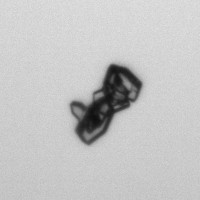
\includegraphics[width=1\linewidth]{figures/litenis1}
  \subcaption{Ice particle.}
  \label{fig:litenis}
\end{subfigure}%
\begin{subfigure}[t]{.5\textwidth}
  \centering
  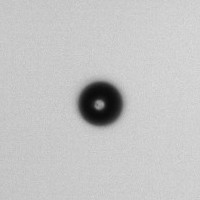
\includegraphics[width=1\linewidth]{figures/litendroppe1}
  \subcaption{Droplet.}
  \label{fig:litendroppe}
\end{subfigure}
\caption{Difference between an ice particle and a water droplet that is 62 µm in diameter. Larger ice and snow particles tend to be more complex in shape. Ice particles smaller than 10 µm in diameter may be difficult to distinguish from water droplets.}
\label{fig:icevsdrop}
\end{figure}

\subsection{Calibration Validation}

The calibration functions derived from the measurement of known sized dots is an approximation and an interpolation. It is based on the assumption that light scatters similarly on the edge independently of the size of the object. This is not quite true, especially for smaller particles \cite{bohr2008}. For particles around ten micrometer or less in diameter we would expect different intensities forming a diffraction pattern close to the edge. The pattern would be stronger the more coherent the illumination. In this system, using LED illumination, the coherence length is short enough that no patterns are visible. Still changes to the edge for the smallest diameters can still not be altogether ruled out.

The experiment using calibrated spheres confirms that the measurement of droplet diameters is accurate. It is however not a confirmation of the measurement volume \cite{ryd2016} since we do not know the concentration of the microspheres. This means that we cannot yet confirm an accurate measurement of the LWC. To do that, an independent verification of the measurement volume is needed.


\section{LED Illumination}

Using a high power LED instead of laser reduces the interference effects used in e.g. holography \cite{henn2013}, but since it is a monochromatic source, interference may not be completely ruled out. The coherence length for the blue LED is calculated in Paper I.

LEDs can sometimes be used with currents far above the specifications, as long as the pulse length is short and the duty cycle is low enough to permit the heat generated to be transported away between the pulses. Using the LED above specifications may though affect the efficiency and aging of the LED. LED emittance also depends on the temperature. Depending on the capacitance of the diode, the rise time may limit the current, although there exist some techniques to shorten the LED pulses \cite{tanaka2011,vele2007}.

The LED used was fully functional after four months of measurements using a current in the short flashes that was 12 times higher than the maximum continous current specified by the manufacturer. At 12 ampere driving current, the flash duration could be lowered to approximately 250 ns, still using the normal settings of amplification in the camera. The LED was not tested in higher currents, but it seems possible that it could work. A question is how high current the LED can handle and how the lifetime is affected by higher driving currents.

\section{Statistics}

A value of both MVD and LWC can be derived from a series of images and since the number of measured droplets will depend on the concentration, the accuracy and precision will depend on the number of samples from the total population of droplets. 

In Paper I we made an estimation of the precision a possible instrument could have using the most ideal scenario, where the ''distribution'' was simulated using a single dot of a known size, measured multiple times. This can be seen as a measure of the highest possible precision, defined by the physical limitations of the system components. The coefficient of variation for the LWC was estimated to 1.6 percent for droplets 25 µm in diameter, and 2.4 percent for droplets 10 µm in diameter. In practice it is difficult to compare this with the measured LWC from a real  distribution of droplets. To know the exact LWC, and measure the same content is practically impossible. 

In Paper III, a comparison is made by measuring polymer microspheres in distributions calibrated by NIST. As can be seen in Table \ref{tab:poly_meas}, the difference between the measured mean diameter and the stated mean diameter is small. This proves that the size measurement is accurate. It was not possible to estimate the concentration of the measured microspheres with the method we used. Possibly a known concentration could be produced in a water dispersion, but then the optical ambient conditions would also be different.


\section{Droplets and Size Distributions}

Droplets that are very close are likely to coalesce, thereby decreasing the number concentration at a rate that appears to increase for larger droplets and more complex droplet size distributions \cite{borda2011}. 

Due to the small depth of the measurement volume, i.e. the measuring range compared with the field of view, the likelihood of finding two droplets very close in the image is very low due to the low number concentration of droplets we are measuring. A solution is to make a measurement of the droplet’s circularity and add this as selection criteria for the measurement. This solution also works as a filter for ice or snow particles. 

The drop size distribution of cloud droplets 3-50 µm in diameter have usually been considered to follow a lognormal or gamma curve \cite{miles2000,lee2010,sein1998}. This also applies to rain \cite{ulb1983}. However, more recent measurements of drop size distributions show that the distribution greatly varies \cite{james2001,shaw2002,peters2005,cob2011}. Consequently, the results will depend on the measurement method and the sampling volume.

\subsection{Sampling Speed and Volume}

Since the DII has no external trigger of the imaging, the sampling speed, i.e. the volume of air and droplets that is scanned per time unit, depends on the measuring volume of each image and the imaging speed. 

The sampling speed of the CDP is linearly dependent on the wind speed. The sample area also depends on the size of the measured droplets, but the factory calibration value is given for all sizes. The sampling speed of the DII depends primarily on the image frame rate and the measurement range for each droplet size. At a wind speed of 2 m/s, the sampling speed of the CDP is $\mathrm{4.1 \cdot 10^{-7} m^{3} \cdot s^{-1}}$. This is 39 times higher than the sampling speed of the DII for 20 µm particles. To achieve the same sampling speed, the frame rate of the DII would need to be almost 200 $s^{-1}$. 

Despite the relatively low sampling speed and the small sampling volume of the DII, it seems that by averaging the LWC and the MVD over a period of 30 minutes, enough precision is achieved to be able to compare the two instruments. Since the purpose of the DII is primarily to detect conditions for icing on wind turbines, and provide in-situ observational data for NWP models, the achieved sampling speed may even be good enough, at least for the latter. If the speed is good enough to decide when to switch on de-icing on the blades depends on how quickly the ice builds up, and what de-icing method is used. During icing, high LWC and high MVD are expected.

When comparing the 30 min moving average values for the period 28 February -- 1 March, shown in Figure \ref{fig:0228-0301_LWCvstime} and Figure \ref{fig:0228-0301_MVDvstime}, there is very good agreement between the curves, with the exception of 11.30-12.00 when at least ten droplets 25-35 um in diameters were measured by the DII, resulting in a significantly higher MVD and LWC measured by the DII than the CDP. The reason why the CDP did not measure any similarly sized particles on this particular occasion is not known. There is also a difference in the MVD when the LWC is very low resulting in a small number of measured droplets.

The sampling speed could be raised by e.g. changing the optical magnification but then at the cost of a lower optical resolving power. Different ideas to increase the sampling speed of the DII are discussed in Paper I and Paper II.

Another way of increasing the sampling speed is to increase the imaging speed. Cameras with a high imaging speed exist and the flash pulse is so short that it would still be a low duty cycle for the LED. The most limiting factor is problably the processing time. This can be solved by implementing parts of the image processing in hardware.

The speed requirement finally depends on the application. If the instrument is used for the verification of NWP models, the sampling speed of the prototype may be enough. If the instrument is supposed to be used for triggering de-icing, the sampling speed may need to be increased.

\subsection{Large Droplets}

The CDP does not measure particles larger than 50 µm. But if the distribution of droplets was following a lognormal, or gamma curve \cite{miles2000,lee2010} also for particles larger than 50 µm, enough large droplets should have been detected by the CDP to see an increase in the measured MVD. As demonstrated, this was not always the case. A possible explanation is that the larger cloud droplets do not follow the lognormal distribution when they are above a certain size. If this is true, the predicted MVD may be less useful for the description of a cloud aerosol distribution, as well as for conclusions about possible icing. In the case with supercooled large droplets, the LWC may be more important to measure than the MVD. But to fully understand this, a parallel measurement using an ice load instrument is required.

Figure \ref{fig:170505_0441_droplet} and Figure \ref{fig:170505_1648_droplet} show supercooled large droplets measured during the fog on 05-02-2017.

\begin{figure}[ht]
  \centering
  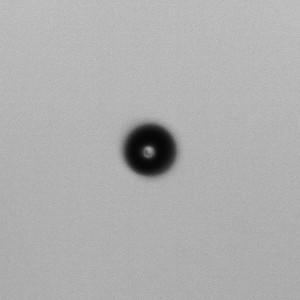
\includegraphics[width=0.4\linewidth]{figures/170205_0441_droplet_74um}
\caption{A 74 µm droplet detected at 04:41 on 05-02-2017.}
\label{fig:170505_0441_droplet}
\end{figure}
\begin{figure}[ht]
  \centering
  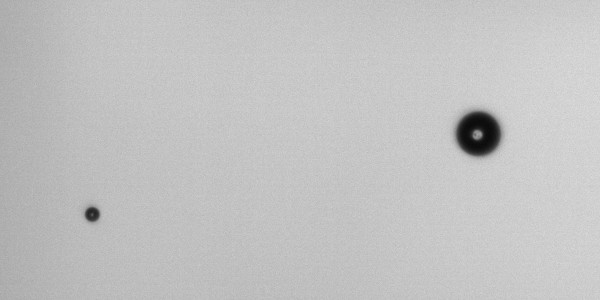
\includegraphics[width=0.8\linewidth]{figures/170205_1648_droplet_19and62um}
\caption{Two droplets, 19 and 62 µm in diameter detected in the same image at 16:48 on 05-02-2017.}
\label{fig:170505_1648_droplet}
\end{figure}


\section{Icing}

The risk of icing increases with increasing wind speed \cite{makk2000}.

During the field study there were several instances when the LWC and MVD was high enough to lead to icing. A study to further investigate the connection between these parameters and the ice load according to ISO 12494 \cite{makk2014} should be carried out. An ice monitoring device, like the Combitech IceMonitor \cite{cost727,thors2015} can be used for this. This should preferably be done in combination with a third independent LWC and MVD measurement, e.g. by using rotating cylinders \cite{makk1992,knez2005}. A heated hygrometer measuring the true water content (\gls{twc}) can be used as an alternative verification of the LWC measurement when all the atmospheric water is in liquid form \cite{spie2012}.






